% vim: tw=78 ai spell spelllang=en

\documentclass[10pt]{llncs}
\usepackage{bold-extra}
\usepackage{xcolor}
\usepackage{url}
\usepackage{graphicx}
\usepackage{listings}
\usepackage{multirow}
\usepackage{xspace}
\pagestyle{plain}

%{{{ (La)TeX definitions

\newcommand\Color[2]{\textcolor{#1}{#2}}
\newcommand{\nb}[1]{\marginpar{\scriptsize #1}}
\renewcommand\note[1]{\nb{\Color{blue}{#1}}}
\newcommand\todo[1]{\nb{\Color{red}{#1}}}
\newcommand\xnote[1]{\Color{green!40!black}{#1}}
\newcommand\snote[1]{\nb{\Color{green!40!black}{#1}}}
\lstset{basicstyle=\ttfamily\scriptsize,escapeinside={(*@}{@*)}}

\newcommand\clang{\textsc{Clang}\xspace}
\newcommand\stanse{\textsc{Stanse}\xspace}
\newcommand\undetI{\textsc{Undetermined I}\xspace}

\newcommand\cdb{\textsc{ClabureDB}\xspace}

%}}}

\begin{document}

%{{{ Title + Author + Abstract

\title{\cdb: Classified Bug-Reports Database}
\subtitle{Tool for developers of program analysis tools}
\author{Jiri~Slaby, Jan~Strej\v{c}ek, and Marek~Trt\'{\i}k}
\institute{Faculty of Informatics, Masaryk University\\
  Botanick\'a 68a, 60200 Brno, Czech Republic\\
  \email{\{slaby,strejcek,trtik\}@fi.muni.cz}}

\maketitle

\begin{abstract}
  We present a database that can serve as a tool for tuning and evaluation
  of miscellaneous program analysis tools. The database contains bug-reports
  produced by various tools applied to various source codes. The bug-reports
  are classified as either real errors or false positives. The database
  currently contains more than 800 bug-reports detected in the Linux kernel
  2.6.28. Support of other software projects written in various programming
  languages is planned. The database can be downloaded and manipulated by
  SQL queries, or accessed via a web frontend.
  % Using the database, developers of various bug-finding tools can easily
  % evaluate effectiveness and performance of their tool.
\end{abstract}

%}}}

%{{{ Intro

\section{Introduction}
\label{sec:introduction}

Many successful bug-finding tools based on various program analysis methods
appeared during the last ten years. None of them is perfect. Each tool
either reports both real errors and false positives, or it discovers only a
part of real errors. To improve or evaluate such a tool, one needs to run
the tool on some source codes and then analyze the obtained bug-reports,
i.e.~classify them as false positives or real errors, and found out errors
in the sources missed by the tool. This work is usually tedious and time
consuming, especially when one tunes or studies performance of a tool for
real software projects.
% , where the number of produced bug-reports can be very high
% (typically hundreds or thousands).

Clearly, there is a serious demand for suitable benchmarks, i.e.~sets of
programs with a (preferably complete) list of their errors. There exist
benchmark suites consisting of small synthetic
programs~\cite{CHK11,CHK09,KRA05,NCH05,SRD} and those consisting of
real-world programs~\cite{CHK09,HW08,LLQ05}. In benchmark
suites~\cite{CHK11,KRA05,NCH05}, relevant program locations in small
synthetic programs are explicitly marked as either erroneous or safe. The
benchmark suite~\cite{CHK09} marks only known real errors. The situation is
different for benchmarks with real-world programs: \cite{LLQ05} contains
marked test cases triggering/non-triggering errors, while~\cite{HW08}
provides bug-reports (both real errors and false positives mixed together)
% without any differentiation)
produced by \textsc{Findbugs} and sorted
according to priority levels assigned to the reports by the tool. The
benchmark suites discussed so far consider different error types and provide
their own error taxonomies with exception of suites \cite{CHK11,CHK09},
where errors types are linked to \emph{Common Weakness Enumeration}
(\textsc{CWE})~\cite{cwe}.

As far as we know, there is no benchmark suite containing big real-life
projects with a significant list of uniformly described bug-reports
classified as real errors or false positive. Our benchmark suite \cdb shoudl
fill this gap. The database currently contains only a single project, namely
the Linux kernel 2.6.28. We have collected over 850 bug-reports of 11 error
types produced by several bug-detection tools run on the kernel. The reports
have been manually classified as either real errors or false positives by
skilled programmers with a help of Linux kernel developers.

The database is still developing in several directions: we plan to add more
bug-reports for the Linux kernel, to support another software project, and
to improve the web interface to allow other users to add and maintain the
database content.

The database can be downloaded in \textsc{SQLite~3} format for a local use
under the \emph{Open Database License v1.0}~\cite{ODbL} or accessed via a
web interface at:
\begin{center}
  \url{http://claburedb.fi.muni.cz/}
\end{center}

\medskip The paper is organized as follows. The following section introduces
the basic structure of the database and our web
interface. Section~\ref{sec:data} describes the current content of the
database including considered kinds of errors and an overview of collected
bug-reports and their sources. Section~\ref{sec:use} suggests possible use
of the database for evaluation of a program analysis tool. Finally, the last
section presents our future plans with \cdb.

%}}}
%{{{ Database Structure

\section{Database Structure}\label{sec:structure}

\begin{figure}[tb]
\begin{center}
\includegraphics[width=\textwidth]{error}
\end{center}
\caption{List of seven bug-reports with one record info expanded.}  
\label{fig:error}
\end{figure}

The database is designed to accommodate various kinds of errors from diverse
projects and their version. As projects can be written in arbitrary
programming languages, can contain very specific kinds of errors, and can be
maintained by and interesting for distinct user groups,
we decided to have each project % and version 
in a separate sub-database. A sub-database comprises information
about considered error types, bug-reports, users, tools, and relations between them. 
There are two main tables in each sub-database:
\begin{description}
\item \textbf{error\_type} This table keeps a specification of considered
  kinds of errors. We will outline some of possible types later in
  Section~\ref{sec:error_type}. The table contains a name of the type, short
  description and a reference CWE number if exists (see later).
\item \textbf{error} Each line in this table corresponds to one
  bug-report. It is specified by the error type, location (usually file and
  line), URL for reference (to provide more info), classification (false
  positive, real error, unclassified), confirmation (an argument supporting
  the validity of the bug-report classification, e.g.~a commit ID of the
  corresponding bug-fix), user who inserted the entry, and timestamp of the
  moment of insertion.
\end{description}

\textbf{
Poznamky:
\begin{itemize}
\item Popsat i dalsi tabulky - nastroje, vztahy nastroj-report, tabulka
  uzivatelu. Mista mame hodne, limit je ted 20 stran LNCS!
\item Chce to obrazek s vice chybama, kde budou i nejaky false positive a
  bude rozbalenej treba druhej zaznam. Obrazek by mel byt citelnejsi
  (doporucuju docasne zvetsit font v .css) a muze byt klidne pres ceou
  stranku.
\end{itemize}
}

Figure~\ref{fig:error} depicts a list of seven bug-reports of type 
\emph{Double Resource Put} as presented in \cdb's web interface at 
\url{http://claburedb.fi.muni.cz/}. Four of these reports are false positives (green),
the other three are real errors (orange). One of the reports is expanded, so that we can see its details and
highlighted source code with a marked error line.

Recall that the database can be also downloaded in \textsc{SQLite~3} format
for a local use under the \emph{Open Database License v1.0}~\cite{ODbL}.

%}}}
%{{{ Current Data and Their Sources

\section{Current Data and Their Sources}\label{sec:data}

\begin{figure}[tb]
\begin{center}
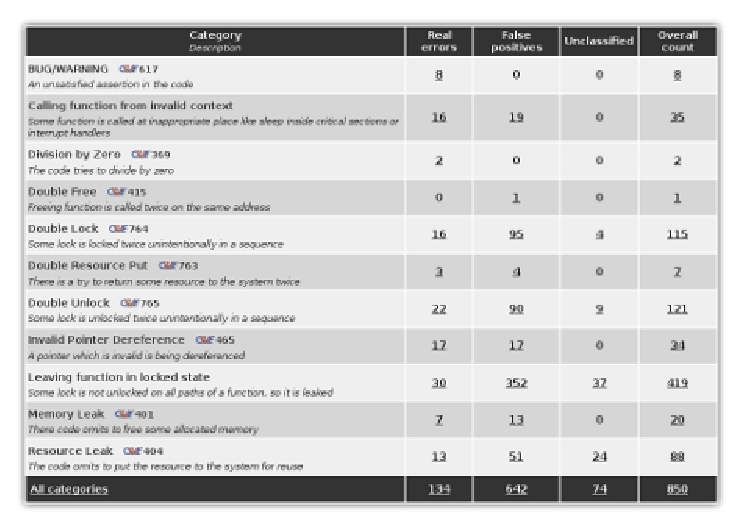
\includegraphics[width=\textwidth]{types}
\end{center}
\caption{Error types in the web interface}
\label{fig:types}
\end{figure}

The benchmark currently contains only bug-reports produced for the Linux
kernel 2.6.28. The following tools were used to gather the bug-reports in that
kernel: \clang~3, \stanse, and one commercial tool which wanted to stay in
anonymity. Note that \clang does not support locking checker for the Linux
kernel natively. We had to slightly modify
\texttt{experimental.unix.PthreadLock} checker just to understand kernel
locking functions. Finally, the database also comprises bug-reports from
kernel and Novell bug tracking systems and mailing lists. For that purpose we
implemented our own web crawler.

\subsection{Linux Kernel Error Types} \label{sec:error_type}
Before we could fill the data in the database, we had to have a set of
error types to put into the \texttt{error\_type} table.  Since there already
exists a publicly available database CWE~\cite{cwe} of error types, we decided
to leverage that. We investigated output of tools we had an output from and
using the CWE database we established a set of error types. Nevertheless, two
of our types are not present in CWE. We consulted their inclusion in CWE, but
it was concluded that they are too project-specific and will not be added.
Here, we list all error types currently available in \cdb. They also form the
title-page of our web-interface as can be seen in Fig.~\ref{fig:types}.

Along with each type below we also attach a remark about the actual error
location. This is to evade a misinterpretation of the error line among
diverse tools and error types. For example an error present at the outgoing
edge of a function may be represented by the opening brace of the function,
closing brace, or by a given \texttt{return} statement. We standardize this
and force tools to provide a line according to this manual. This way we can
compare the reports and remove potential duplicates.

\begin{description}
\item \textbf{BUG/WARNING} (CWE 617)
Developers often inject \emph{assert}s to their code, e.g.~to ensure the input
to their function is as they intended. Sometimes however, these assertions are
hit and crashes enforced. A typical use case might be when we implement a
destroy function of an object and we want to enforce the caller (by a crash)
to make the object dead prior calling our function. In that case a check like
\texttt{assert(!obj->active)} will do the work. \\
The error location is the line where the assertion appears in the code.

\item \textbf{Division by Zero} (CWE 369)
The code contains a division instruction but the actual value of the divisor
is zero. \\
The error location is the line where the division appears in the code.

\item \textbf{Double Lock} (CWE 764)
Some lock is locked by a thread twice in a row and it leads to an inconsistent
lock state. Note we exclude intentional double locks of semaphores where this
may not be an issue.  \\
The error location is the line with the second call of lock.

\item \textbf{Double Unlock} (CWE 765)
Some lock is unlocked by a thread twice in a row and it leads to an
inconsistent lock state. \\
The error location is the line with the second call of unlock.

\item \textbf{Double Free} (CWE 415)
A freeing function is called twice on the same address while no reassignment
to the passed pointer occurred. Most allocators can detect this and usually
kill the program. \\
The error location is the line of the invalid (second) free.

\item \textbf{Memory Leak} (CWE 401)
Some code omits to free a memory which was allocated previously. \\
The error location is the line where the allocation occurs.

\item \textbf{Invalid Pointer Dereference} (CWE 465)
The code tries to access some memory, but the pointer used is invalid. It may
become invalid by many ways. Be it using of memory which was freed by other
part of the system or driver, be it forgotten initialization of some pointer
(it is NULL or undefined value). Also the source of the problem might be
accessing an array out of bounds. \\
The error location is specified by the line of the dereference.

\item \textbf{Double Resource Put} (CWE 763)
The code requests one copy of a resource (e.g.~a structure holding hardware
status) from a system, but there is more than one attempt to put that resource
back to the system. Like in this example:
\begin{lstlisting}[language=C]
struct pci_dev *pdev = pci_get_device(vendor, device, NULL); // get
if (pdev) {
  work_with_pdev(pdev)
  pci_dev_put(pdev);               // first put
}
pci_dev_put(pdev);                 // second (illegal) put of the same
\end{lstlisting}
The error location is the line of the second put.

\begin{table}[tb]
\begin{center}
\small
\setlength{\tabcolsep}{2.5pt}
\begin{tabular}{|l|c|c|c|c|} \hline
\textbf{Error Type} & \textbf{Real Err.} & \textbf{False Pos.} &
	\textbf{Unclassified} & \textbf{Total} \\ \hline

BUG/WARNING & 8 & 0 & 0 & 8 \\
Calling function from invalid context & 16 & 19 & 0 & 35 \\
Division by Zero & 2 & 0 & 0 & 2 \\
Double Free & 0 & 1 & 0 & 1 \\
Double Lock & 16 & 95 & 4 & 115 \\
Double Resource Put & 3 & 4 & 0 & 7 \\
Double Unlock & 22 & 90 & 9 & 121 \\
Leaving function in locked state & 30 & 352 & 37 & 419 \\
Memory Leak & 7 & 13 & 0 & 20 \\
Invalid Pointer Dereference & 17 & 17 & 0 & 34 \\
\hspace{1em}{\scriptsize NULL Pointer Dereference} & 17 & 14 & 0 & 31 \\
\hspace{1em}{\scriptsize Use After Free} & 0 & 3 & 0 & 3 \\
Resource Leak & 13 & 51 & 24 & 88 \\ \hline

\textbf{Overall Count} & 134 & 642 & 74 & 850 \\ \hline
\end{tabular}
\end{center}
\caption{Reports in \cdb.}
\label{tab:reports}
\end{table}

\item \textbf{Resource Leak} (CWE 404)
The code requests a resource from a system, but omits to return that back.  In
the previous example, both \texttt{pci\_dev\_put} calls would be missing.  \\
The error location is the line of the request/get.
\end{description}

The following two error types may be only Linux kernel specific. Note that the
database is not limited to a bounded set of error types. Each project may
extend this set by arbitrary error types.

\begin{description}
\item \textbf{Calling function from invalid context} (not in CWE)
Some function is called at inappropriate place or within an invalid context.
This includes calling functions like sleep or wait inside spin-lock critical
sections or in interrupt handlers. If that happens, results are undefined, the
system may become unresponsive or may crash for instance. \\
The error location is the line of the inappropriate call.

\item \textbf{Leaving function in locked state} (not in CWE)
There is a path in a function where some lock is locked but unintentionally
left locked when returning from the function. This often results in deadlocks
on next invocation of any function wanting to take the same lock. This error
type originates from the kernel requirements when returning to userspace a
process cannot hold any locks. And yet, this is sometimes reported by tools
which analyze a large project per module and start the analysis from some
chosen starting functions.  If the lock is locked while leaving these initial
functions, the tools generate this report.  \\
The error location is the line of \texttt{return} statement or closing brace
if there is no \texttt{return}.
\end{description}

\subsection{Errors}
The database comprises 850 reports: 134 real errors, 642 false positives, and
74 entries which are unclassified. Many of the unclassified entries were
added even recently and are about to be classified soon.
Table~\ref{tab:reports} depicts how each kind of bugs is represented in the
database.

Further, we used our database for comparing kernel subsystems according to
error occurrence in Table~\ref{tab:stats}. For the presentation purposes we
excluded subsystems with less than 10 reports. Those were security,
virtualization, or inter-process-communication subsystems for example. Based
on the findings of the tools we used, we can see that the highest ratio of
errors per file is in the sound subsystem and a core code performing memory
management and maintaining running system. On the other hand we see that the
tools were very unsuccessful to find real errors in networking subsystem while
they found relatively many false positives there. The core is the worst
written code with respect to the tools in this manner. In average, every
second file contained a false positive.

What is not in the Table~\ref{tab:stats}, but can be pulled out of \cdb is that
maximum false positives per file (19) is found in the very core of the kernel
scheduler in \texttt{kernel/sched.c}. It is followed by the XFS filesystem in
\texttt{fs/xfs/xfs\_log.c} with 14 hits and directory cache management in
\texttt{fs/dcache.c} with 12 hits. All of them but two are related to improper
locking. In most of the cases, the false positives stem from too complex code.
The tools could not often cope with a conditional call to lock and yet,
located in a loop.

\begin{table}[tb]
\begin{center}
\setlength{\tabcolsep}{2.5pt}
\begin{tabular}{|l|c|c|c|c|c|c|} \hline
\textbf{Subsystem} & \textbf{Files} & \textbf{KLOC} & \textbf{Real Err.} &
	\textbf{False Pos.} & \textbf{Errs/file (\%)} & \textbf{FPs/file (\%)} \\ \hline

Arch        &  354 &  146 &  6 &  15 & 1.69 & 4.24 \\
Core        &  202 &  166 &  5 & 104 & 2.48 & 51.49 \\ % mm+kern
Drivers     & 4492 & 4029 & 88 & 205 & 1.96 & 4.56 \\
Filesystems &  899 &  720 & 16 & 164 & 1.78 & 18.24 \\
Networking  &  834 &  525 &  5 & 127 & 0.60 & 15.22 \\
Sound       &  529 &  438 & 13 &  10 & 2.46 & 1.89 \\ \hline

\textbf{Summary} & 7310 & 6960 & 133 & 625 & 1.82 & 8.55 \\ \hline
\end{tabular}
\end{center}
\caption{Statistics}
\label{tab:stats}
\end{table}

%}}}
%{{{ Intended Use of the Database

\section{Intended Use of the Database [TOHLE NENI DODELANY]}\label{sec:use}

To evaluate a bug-finding tool, one can analyse a project from our benchmark
suite and compare the produced bug-reports to those in the database. This way,
one immediately gets a classification (real error/false positive) of the
reports matched in the database and also information about some missed real
errors. This information can be further statistically processed according to
methodologies of~\cite{CHK09,HW08}.

\begin{itemize}
\item run your tool
\item compare outgoing bug reports against the database, get the information
  which reports correspond to a real bug and which are false positives
\item classify the rest of your error reports
\item update the database and evaluate the tool (also in terms of real
  errors not find by the tool)
\end{itemize}

%}}}
%{{{ Future Plans

\section{Future Plans}

We plan to extend the database in several directions. Namely, we intend to
collect more bug-reports and to support more error types in the current
project. Further, we want to add other real-life projects. We also plan to
extend the web interface to enable other users to maintain and extend the
database. The future of our database depends also on a feedback of the
program analysis community. Hence, if you have any suggestions, source of
bug-reports, or another comments, please contact us at
\texttt{claburedb@fi.muni.cz}.

\todo{Interface for insertion is under construction.}
\todo{Emphasize openness.}
\todo{file+line tuples}
\todo{emphasize genuineness of errors}
\todo{novelty is not only the false-positives, but also the contents}
\todo{related work?}

%}}}

\bibliographystyle{plain}
\bibliography{bd}

\end{document}

%{{{ MARKOVO

\clearpage
\section{Related Work}

There are benchmark suites consisting of small synthetic
programs~\cite{CHK09,KRA05,CHK11,NCH05,SRD} and those consisting of real-world
programs~\cite{CHK09,LLQ05,HW08}. Bug-reports in small synthetic programs are
explicitly marker as either real errors or false positives in benchmark
suites~\cite{KRA05,CHK11,NCH05}. The benchmark suite~\cite{CHK09} marks only
real errors. In case of real-world programs the situation is different. Real
errors and false positives are identified in~\cite{LLQ05} by constructed test
cases hitting or missing known errors, and in~\cite{HW08} there the
bug-reports are collected from \textsc{Findbugs} and sorted according to
priority levels assigned to the reports by the tool. The benchmark suites
discussed so far considers different error types and provide their own error
taxonomies. An exception is~\cite{CHK11}, where errors types are linked to
\textsc{CWE}~\cite{cwe}.

Our benchmark suite \cdb differs from the previous approaches, since it
provides correct and explicit marking of both real errors and false positives
in real-world programs. In addition, \cdb provides linking of error types to
\textsc{CWE}~\cite{cwe}. Its goal is to provide tuning data for later stages
of development of program analysis tools. Therefore, \cdb fills the gap in
services provided by benchmark suites of the previous approaches.

\subsection{Notes (they are not meant to appear in the article)}\label{sec:relwork:notes}

\subsubsection{(1) BegBunch -- Benchmarking for C Bug Detection Tools~\cite{CHK09}} This benchmark suite consists of two suites of different purpose. The \emph{Accuracy suite} consists of small benchmarks, called bug-kernels, which were extracted from existing buggy open source applications, like OpenSolaris or MySQL. The bug-kernels was extracted by inspecting bug tracing systems and mailing lists. The bug-kernels contains errors of the following types: buffer overflow, memory/pointer issues, integer overflow, and format string. Each bug in a bug-kernel is annotated with an XML-like markup of the same line that exposes the bug. The second suite \emph{Scalability suite} is composed of a particular versions of several open source applications (like MySQL 5.0.51a, Perl 5.8.4, Sendmail 8.12.3, etc.) of various size from small to large. There is no bug-reports considered in this suite. Only size of benchmarks is considered. The purpose of this suite is to measure how well a program analysis tool scales in spite of size of an analysed code.

\subsubsection{(2) BugBench: Benchmarks for Evaluating Bug Detection Tools~\cite{LLQ05}} Benchmarks are in the form of complete program distributions. It is composed of 17 programs (like gzip-1.2.4, cvs-1.11.4, msql-4.1.1, etc.) including 19 bugs (like stack smash, global buffer overflow, heap buffer overflow, uninitialised read, memory leak, double free, data race,  atomicity, and semantic bug) that were known to exist in these programs. BugBench provides test cases, both triggering and non-triggering bugs known in the programs. They do not mark false positives in the programs.

\subsubsection{(3) On Establishing a Benchmark for Evaluating Static Analysis Alert Prioritization and Classification Techniques~\cite{HW08}} Benchmarks of our FaultBench benchmarks suite are in the form of complete Java program distributions (like jbook 1.4, jdom 1.1, xmlwriter 2.2.2, itrust fall 2007) including known bugs. FaultBench evaluates static analysis false pasitive mitigation techniques. The goal is to find best false positive mitigation technique with best rate of anomaly detection.

\subsubsection{(4) Using a Diagnostic Corpus of C Programs to Evaluate Buffer Overflow Detection by Static Analysis Tools~\cite{KRA05}} The corpus consists of 291 small C programs generated in four versions: with no buffer overflow, and with minimum, medium, and large buffer overflows. This corpus is dedicated to check buffer overflow errors.

\subsubsection{(5) Test-driving static analysis tools in search of C code vulnerabilities~\cite{CHK11}} The benchmarking test suite includes more than 700 programs, where each of them consists from 10 to 100 lines of code. All programs have a line with the tested flaw commented as /*ERROR*/ and another line commented as /*SAFE*/ that checks the tool capability to avoid reporting spurious errors. Error types used in the benchmarks have their links (IDs) to CWE.

\subsubsection{(6) ABM: A Prototype for Benchmarking Source Code Analyzers~\cite{NCH05}} The benchmark test suite is composed of 91 micro-benchmark C test cases. Whenever possible, test cases were constructed in matched pairs of OK and BAD test cases. Each BAD
test case has code with a vulnerability in it. Corresponding OK cases are similar to BAD cases but do not share the vulnerability. OK cases are generally constructed by patching. Each test case contains annotations specifying where a bug may be present. Test cases with vulnerabilities are tagged with a comment “/* BAD */” at any line that may be considered to contribute to the vulnerability described by the test case’s keywords. Those cases without vulnerabilities are tagged with a comment “/* OK */” at any line that could have contributed to the vulnerability if it had been present. Each test case is also annotated with information about valid and invalid inputs.

\subsubsection{(7) CVE and CWE~\cite{cwe}} These are just errors taxonomies.

\subsubsection{(8) NIST SAMATE Reference Dataset~\cite{SRD}} It is a suite of synthetic benchmarks  mainly for C, C++, and Java, that have been contributed by various groups. Ignore this...probably.

\subsubsection{SPEC} Ignore this...probably.

\subsubsection{TCP} Ignore this...probably.
\clearpage
\subsubsection{*** Classification of the approaches above ***}
\begin{description}
  \item[Those containing small synthetic programs] \cite{CHK09}, \cite{KRA05}, \cite{CHK11}, \cite{NCH05}, \cite{SRD}

  \item[Those containing big programs] \cite{CHK09}, \cite{LLQ05}, \cite{HW08}

  \item[Those marking errors in small programs] \cite{CHK09}, \cite{KRA05}, \cite{CHK11}, \cite{NCH05}

  \item[Those marking errors in big programs] \cite{LLQ05} by test cases hitting known errors, \cite{HW08} only reports classified by Findbugs tool

  \item[Those marking false positives in small programs] \cite{KRA05}, \cite{CHK11}, \cite{NCH05}

  \item[Those marking false positives in big programs] \cite{LLQ05} by test cases missing known errors, \cite{HW08} only reports classified by Findbugs tool

  \item[Those who reference CVE/CWE] \cite{CHK09,CHK11}

  \item[Those containing no programs, only classifies error types] \cite{cwe}
\end{description}

%}}}

\end{document}

%{{{ Intro

\section{Introduction}
\label{sec:introduction}

databaze klasifikovanych chyb pro ladeni toolu urcenych pro analyzu realneho kodu.
availability, related work, url,

\xnote{
Nasledujici ctyri body predstavuji vecny obsah teto sekce. Dulezite je i jejich poradi. (nejen v techto bodech pouzivam tyto zkratky: Sorted Bug-reports Database (SBD), Program Analysis Tool (PAT)).
\\
(1) Problem pri vyvoji PATu, ktery zde hodlame resit:
%
Zamerujeme se na takove PATy, ktere mohou pri sve cinnosti produkovat falesna hlaseni. Uvest priklady takovych PATu (BLAST, SLAM, SDV, COVERITY, KLOCWORK, XGCC, CPPCHECK, PREFIX, PREFAST, ...).
%
Jde nam o pozdejsi stadia vyvoje techto PATu, kdy se ma nastroj zacit vyhodnocovat na realnych programech.
%
PAT pusteny na realnem programu casto generuje velke mnozstvi bug-reportu, o kterych predem nevime, ktere reporty predstavuji realne chyby, a ktere jsou jen falesna hlaseni. Zduraznit, ze overovani chyby/falesneho hlaseni v realnem, cizim a neznamem kodu je casto casove narocna a nezaziva prace.
%
Cilem SBD je tuto casove narocnou a nezazivnou cinnont znacne redukovat.
\\
(2) Jak konkretne SBD pomuze pri trideni bug-reportu:
%
SBD obsahuje pro analyzovany program velke mnozstvi jiz drive roztridenych bug-reportu. Vyvojari PATu tak staci, aby porovnal vystup z jeho toolu s obsahem SBD.
%
Krome vlastniho roztrideni (velke) casti vsech bug-reportu PATu na realne chyby a false positiva, vyvojar dale ziska prehled o znamych realnych chybach, ktere jeho PAT v analyzovane casti programu prehledl.
\\
(3) Prirozene zkvalitnovani SBD:
%
Muze se stat, ze vyvijeny PAT vyprodukuje na danem programu bug-report, ktery doposud neni v SBD. Vyvojar muze tento bug-report vlozit do SBD a muze k nemu pripojit informaci o tom, jestli jde o realnou chybu nebo o falesne hlaseni. Timto prispivanim do SBD si mohou vsichni vyvojari PATu vzajemne setrit cas.
%
SBD je navic navrzena tak, ze se do ni daji vkladat ruzne programy a dokonce i ruzne jejich verze. SBD tak mohou vyuzit i PATy specializovane na urcite typy programu (napr. na knihovny pro praci s retezci, sobory, GUI, apod.).
\\
(4) Statisticke udaje o cinnosti PATu na danem programu pomoci SBD: Uzivatel by mel mit moznost si v SBD oznacit moduly z daneho programu (verze), ktere jeho PAT analyzoval. Pak by mel mit moznost oznacit v SBD, ktere bug-reporty jeho PAT vyprodukoval. SBD by mu pak mela poskytnout statistiku, kolik nasel realnych chyb toho ktereho typu, kolik mel falesnych hlaseni toho ktereho typu, procentualni zastoupeni falesnych hlaseni, apod. 
}

There are several successful tools for finding errors in real code like
\textsc{Coverity}~\cite{coverity}, or \stanse~\cite{stanse}.
It is quite common that these tools generate, besides the errors which can
really occur during the execution, also false positives. Mostly, implementers
of such tools have to sort these reports manually to have an overview of how
the tool stands amongst others. To alleviate this burden, we augmented this
idea. We fixed a project and version and created a database of marked errors
where everybody may come and compare their tool. This will immediately return
count of errors the tool found along with false positives count. But more
importantly, it will tell the implementers also the count of errors that were
completely missed by their tool.

There were attempts to create a similar database previously like
in~\cite{IBM_database}. However those were either built upon a synthetic code
base, tailor-made exactly for that purpose, or they did not meet with success
because they have not got enough errors in the data base.

We built our database on the Linux Kernel. The idea behind is to have a real,
large-scale code base which might be also easily obtained. The version we
chose is a couple of years old version 2.6.28. The elderly version has several
reasons. First, we do not want to expose security holes of some new kernel to
wide public. Second, more importantly, we have an input from the kernel
developers on this particular version for all reports of chosen tools, so that
we are sure which errors are real and which are not.

In the end the database comprises 474 reports in 11 categories. The most
investigated categories from our side are locking errors like \emph{double
lock}, \emph{double unlock} or \emph{leaving functions in locked state}.
These are from the output of \stanse, \sparse\note{fakt?}, and
one tool from a North-American company dealing with static analysis of the
Linux kernel, we call this \undetI.

%}}}
%{{{ Marek

\section{\xnote{Sorted Bug-reports Database}}

\subsection{\xnote{Usage}}

\xnote{
V teto subsekci predvedeme, jak se konkretne s SBD pracuje. Jako PAT zvolime STANSE a budeme tridit jeho vystup (bug-reporty) pomoci SBD. Jednotlive ukazky budou zcela konkretni realne priklady pouziti SBD, ktere si kdokoliv muze sam hned odzkouset. Predvedeme nasledujici veci:
\\
(1) Trideni bug-reportu z PATu pomoci SBD: (a) Pomoci SQL dotazu: Vezmu nejakou vhodnou hlasku ze STANSE a ukazu SQL dotaz do SBD, ktery vrati, zda se jedna o chybu nebo falesne hlaseni, nebo ze hlaska zatim neni v SBD. Klidne lze udelat 3 priklady pro jednotlive mozne vysledky. Vhodne by mohly byt obrazky vystupu z konzole apod. (b) Pomoci weboveho rozhrani: Provedu totez co v (a), akorat zde zobrazim prislusne nastavena GUI okenka z weboveho rozhrani.
\\
(2) Pridani noveho bug-reportu do SBD: (a) Pomoci SQL dotazu: Vezmu nejakou vhodnou hlasku ze STANSE (nejlepe tu z tech 3 hlasek z bodu (1)) a ukazu SQL dotaz do SBD, ktery zajisti vlozeni bug-reportu do SBD. Mely by se odiskutovat jednotlive varianty dotazu (napr. vlozeni rovnou s klasifikaci bug/false alarm; dale typ chyby; pridani dalsich doplnujicich dat k zaznamu). (b) Pomoci weboveho rozhrani: Provedu totez co v (a), akorat zde zobrazim prislusne nastavena GUI okenka z weboveho rozhrani.
\\
(3) Pridani noveho programu, ci verze do SBD: (a) Pomoci SQL dotazu: Zvolim nejaky (mensi) open source a program ci knihovnu (pak se domluvime, co by to tak asi mohlo byt) a jeho/jeji nejakou verzi a formuluji SQL dotaz, ktery vlozi ten program do SBD. (b) Pomoci weboveho rozhrani: Provedu totez co v (a), akorat zde zobrazim prislusne nastavena GUI okenka z weboveho rozhrani. Mimochodem, tento bod (3) se da cely take zatim vyresit tak, ze rekneme, ze tato funkcionalita je prozatim ve vyvoji, ale bude zpristupnema v blizke budoucnosti.
\\
(4) Statisticke udaje o cinnosti PATu na danem programu pomoci SBD: (a) Pomoci SQL dotazu: Vzal bych vystup STANSE na urcitych par modulech. Pro tento vystup bych formuloval ruzne varianty SQL dotazu do SBD pro ziskani ruznych statistickych udaju o analyze. Mel by se take odiskutovat ten univerzalni format zadavani bug-reportu v dotazu a format seznamu analyzovanych modulu. (b) Pomoci weboveho rozhrani: Provedu totez co v (a), akorat zde zobrazim prislusne nastavena GUI okenka z weboveho rozhrani.
}

%}}}
%{{{ Results

%\section{Results}
\subsection{\xnote{Current State}}

\xnote{
Zde bych dal vsechny zajimave statisticke udaje o aktualnim stavu obsahu SBD. Nezapomenout uvest verzi kernelu, kterou tam mame. Take odiskutovat propojeni s tou databazi nejcastejsich chyb v SW (nemuzu si vzpomenout na tu zkratku) a diskuse zvolenych typu chyb v SBD. Sekci bych uzavrel nasimi plany s SBD do blizke budoucnosti (neco jako kratka Future Work).
}


\stanse, by its nature of overapproximating, reported all the reports.
\undetI failed to report 46\todo{exact count needed}. We
believe this is because of the default settings of the tool or due to filters
which are executed on the analysis results.

\subsection{\xnote{Availability}}

\xnote{
Krome vlastniho URL bych zde zminil moznost stazeni SBD (s licencnimi podminkami, pripadne) pro praci off-line. Pro tuto moznost stazeni SBD je ale nutne dodat na webove stranky instalacni manual. Zde muzeme navic pripadne dat odkaz na tuto stranku. Dale musime zminit, ze subsekce Usage obsahuje konkretni priklady pouziti, ktere je mozne na dane URL primo odzkouset. A ze z te sekce by take melo byt zcela jasne, jak pri zkouseni postupovat (tj. sekci lze tez chapat jako manual pro pouziti tech prikladu).
}

%}}}
%{{{ Conclusion

\paragraph{Acknowledgements}
\label{sec:acknowledgements}

Jan Strej\v{c}ek has been supported by The Czech Science Foundation
(GA\v{C}R), grants No.~P202/10/1469 and P202/12/G061. Ji\v{r}\'i Slab\'{y}
and Marek Trt\'{\i}k have been supported by The Czech Science Foundation
(GA\v{C}R), grant No.~102/09/H042.

%}}}

\bibliographystyle{plain}
\bibliography{bd}

%%% Local Variables: 
%%% mode: latex
%%% TeX-command-default: "pdfLaTeX"
%%% End: 
